\begin{frame}[allowframebreaks]{Learning Ensembles}
    \begin{itemize}
        \item \textbf{Learn multiple trees and combine their predictions}
        \begin{itemize}
            \item Fix overfitting/underfitting problem in decision trees
            \item Gives better performance in practice
            \item The “wisdom of the crowds”
        \end{itemize}

        \item \textbf{The parable of the ox (Sir Francis Galton, 1906)}
        \begin{itemize}
            \item 787 people guessed the weight of an ox
            \item Avg crowd guess: 1,197 pounds
            \item True weight: 1,198 pounds
        \end{itemize}
    \end{itemize}

    \begin{center}
        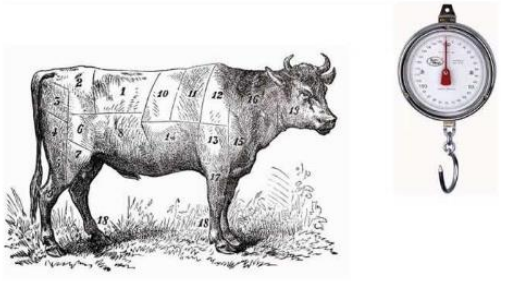
\includegraphics[width=0.4\textwidth]{images/decision-trees/decision-trees-13.png}
    \end{center}
\end{frame}


\begin{frame}[allowframebreaks]{Learning Ensembles}
    \textbf{Bagging (bootstrap aggregation):}
    \begin{itemize}
        \item Learns multiple trees \underline{in parallel} over independent samples of the training data
        \item \textbf{1) Bootstrapping:} Given a dataset $D$ on $n$ data points: Create multiple datasets $D'$ of $n$ points by sampling from $D$ with replacement:
        \begin{itemize}
            \item 37\% points in $D'$ will be duplicates, 63\% will be unique
        \end{itemize}
        \item \textbf{2) Parallel training:} Train decision trees on samples independently and in parallel
        \item \textbf{3) Aggregation:} Depending on the task, an average or majority of the predictions are computed for a more accurate estimate
    \end{itemize}
\end{frame}


\begin{frame}[allowframebreaks]{(1): Bagging Decision Trees}
    \begin{center}
        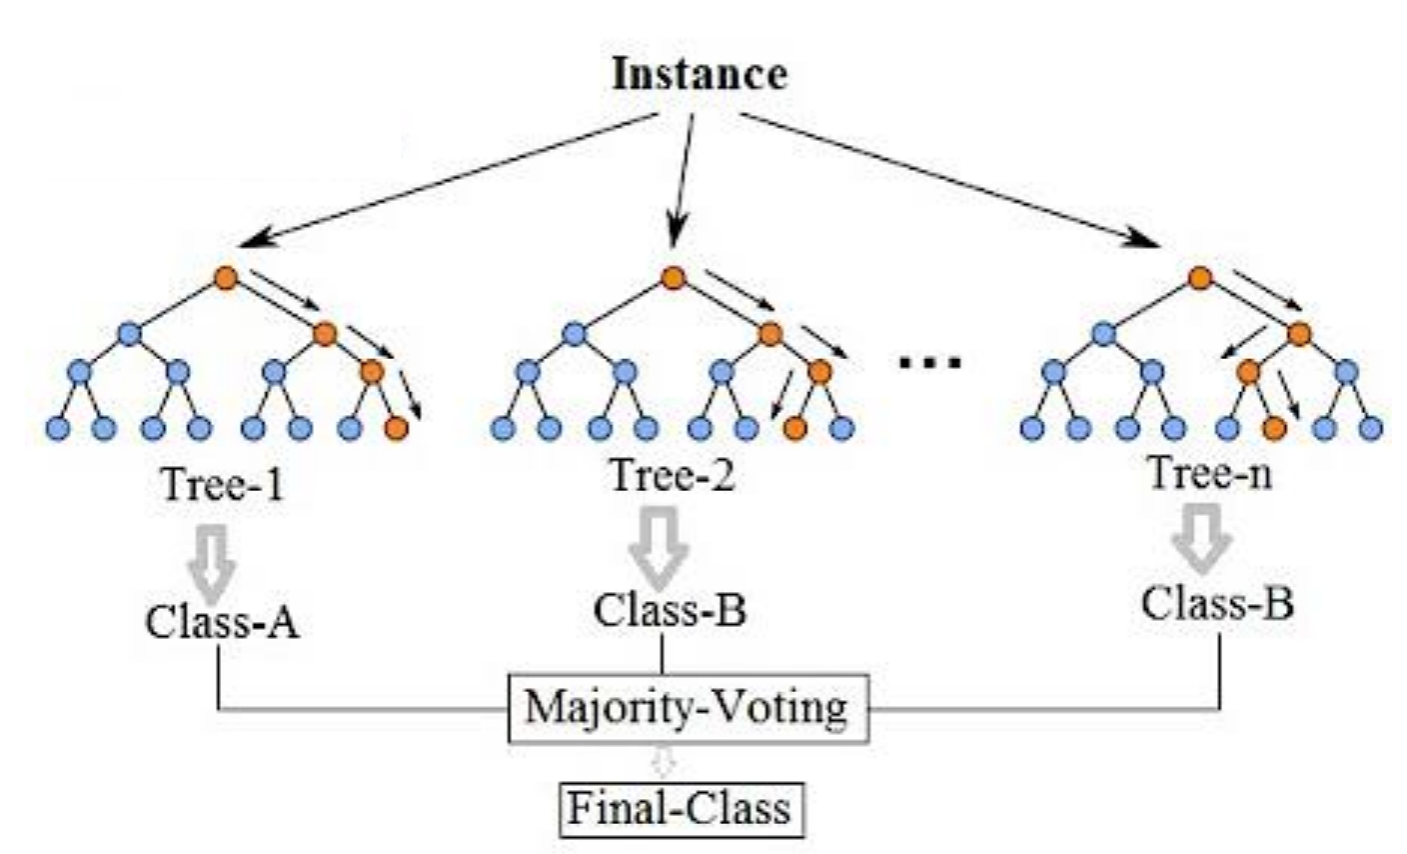
\includegraphics[width=0.95\linewidth]{images/decision-trees/decision-trees-14.png}
    \end{center}
\end{frame}

\begin{frame}[allowframebreaks]{(1): Instance Bagging}
\begin{itemize}
    \item Decision trees are greedy
    \begin{itemize}
        \item They choose which variable to split on using a greedy algorithm that maximizes purity or information gain
    \end{itemize}
    \item Even with Bagging, the decision trees can have a lot of structural similarities and correlation in their predictions
    \begin{itemize}
        \item If one feature is very strong predictor, then every tree will select it, causing trees to be correlated.
    \end{itemize}
    \item But ensemble learning works best with independent predictors
\end{itemize}
\end{frame}

\begin{frame}[allowframebreaks]{(2) Improvement: Random Forests}
\begin{itemize}
    \item Train a Bagged Decision Tree
    \item But use a modified tree learning algorithm that selects (at each candidate split) a random subset of features
    \begin{itemize}
        \item If we have $d$ features, consider $\sqrt{d}$ random features
    \end{itemize}
    \item This is called: Feature bagging
    \begin{itemize}
        \item Benefit: Breaks correlation between trees
    \end{itemize}
    \item Random Forests achieve state-of-the-art results in many classification problems!
\end{itemize}
\end{frame}

\begin{frame}[allowframebreaks]{(3): Boosting}
\begin{itemize}
    \item \textbf{Boosting:} Another ensemble learning algorithm
    \begin{itemize}
        \item Combines the outputs of many ``weak'' classifiers to produce a powerful ``committee''
        \item Learns multiple trees sequentially, each trying to improve upon its predecessor
        \item Final classifier is weighted sum of the individual classifiers
    \end{itemize}
\end{itemize}

\begin{figure}[h]
    \centering
    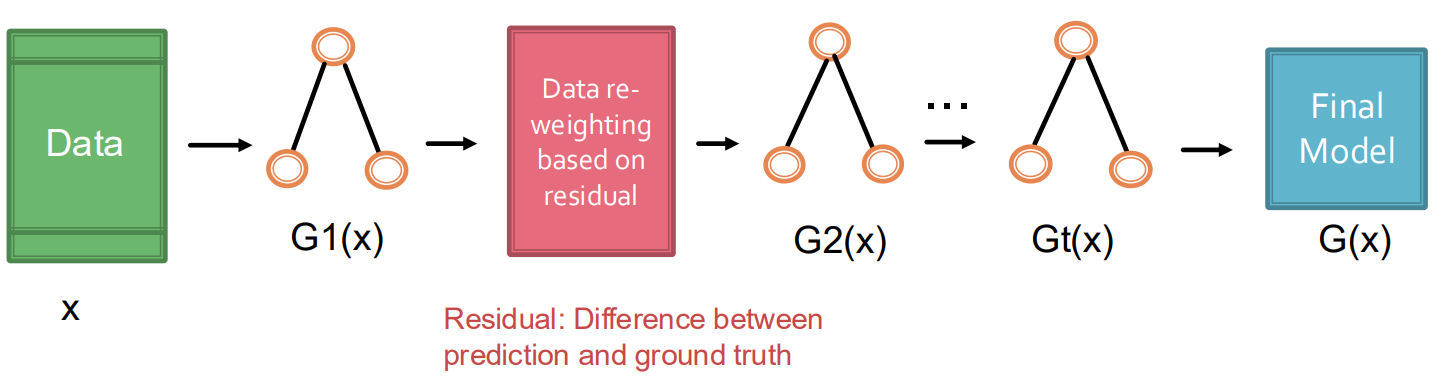
\includegraphics[width=0.9\textwidth]{images/decision-trees/decision-trees-15.png}
\end{figure}

\end{frame}


\begin{frame}[allowframebreaks]{(3): Boosting}
\begin{itemize}
    \item \textbf{We will show 2 examples:}
    \begin{itemize}
        \item \textbf{Example 1: AdaBoost}
        \begin{itemize}
            \item Where each $G_t(x)$ is a one-level decision tree
        \end{itemize}
        \item \textbf{Example 2: Gradient Boosted Decision Trees}
        \begin{itemize}
            \item Where each $G_t(x)$ is a multi-level decision tree
        \end{itemize}
    \end{itemize}
\end{itemize}

\begin{figure}[h]
    \centering
    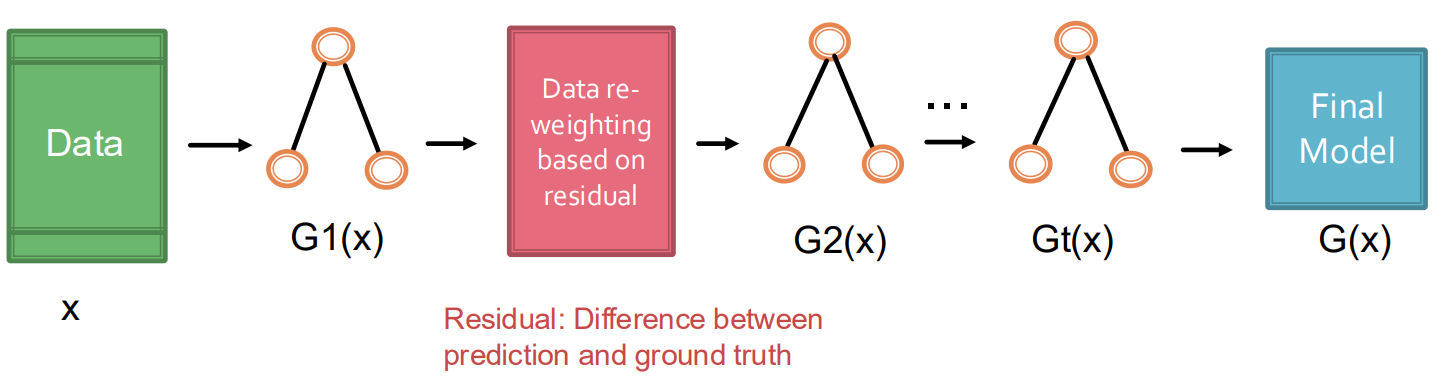
\includegraphics[width=0.9\textwidth]{images/decision-trees/decision-trees-15.png}
\end{figure}

\end{frame}
